% questions.tex —— 2014 年全国Ⅰ卷（理科） · 题目内容片段（无答案）
% 由 tools/generate_projects.py 依来源总账自 2014/2014_数学真题_全国1理_试题.md 生成，勿手改（改源 MD 后重跑）


\gkpart{数学}

\begin{gktip}
\textbf{来源说明}：本题面依据固定源 PDF 两页 A3 题面逐题转录，原卷印刷页码 899–900。固定源只含试题和作答空白，不附答案或解析；答案和解析均由本库独立复算。

\textbf{图形说明}：第 6、7、12、18、19、22 题的题面图形在 LaTeX 工程中以 TikZ/PGFPlots 矢量源重绘。题面中的图片标记仅为转换器定位这些矢量源的标记，仓库不保存 PNG、JPEG 或 SVG 图形文件。
\end{gktip}

\gkpart{一、选择题}

\begin{question}
\gkti{1}已知集合 $A=\{x\mid x^2-2x-3\geqslant0\}$，$B=\{x\mid-2\leqslant x<2\}$，则 $A\cap B=$\mbox{（　　）}

（A）$[-2,-1]$　　（B）$[-1,2)$　　（C）$[-1,1]$　　（D）$[1,2)$

\end{question}
\begin{question}
\gkti{2}$\dfrac{(1+i)^3}{(1-i)^2}=$\mbox{（　　）}

（A）$1+i$　　（B）$1-i$　　（C）$-1+i$　　（D）$-1-i$

\end{question}
\begin{question}
\gkti{3}设函数 $f(x),g(x)$ 的定义域都为 $\mathbb R$，且 $f(x)$ 是奇函数，$g(x)$ 是偶函数，则下列结论正确的是\mbox{（　　）}

（A）$f(x)g(x)$ 是偶函数　　（B）$|f(x)|g(x)$ 是奇函数

（C）$|g(x)|f(x)$ 是奇函数　　（D）$|f(x)g(x)|$ 是奇函数

\end{question}
\begin{question}
\gkti{4}已知 $F$ 是双曲线 $C:x^2-my^2=3m (m>0)$ 的一个焦点，则点 $F$ 到 $C$ 的一条渐近线的距离为\mbox{（　　）}

（A）$\sqrt3$　　（B）$3$　　（C）$\sqrt{3m}$　　（D）$3m$

\end{question}
\begin{question}
\gkti{5}$4$ 位同学各自在周六、周日两天中任选一天参加公益活动，则周六、周日都有人参加公益活动的概率为\mbox{（　　）}

（A）$\dfrac18$　　（B）$\dfrac38$　　（C）$\dfrac58$　　（D）$\dfrac78$

\Needspace{0.4\textheight}
\end{question}
\begin{question}
\gkti{6}如图，圆 $O$ 的半径为 $1$，$A$ 是圆上的定点，$P$ 是圆上的动点，角 $x$ 的始边为射线 $OA$，终边为射线 $OP$，过点 $P$ 作直线 $OA$ 的垂线，垂足为 $M$，将点 $M$ 到直线 $OP$ 的距离表示为 $x$ 的函数 $f(x)$，则 $y=f(x)$ 在 $[0,\pi]$ 上的图象大致为\mbox{（　　）}
\nopagebreak[4]
\begin{center}% 2014 全国卷Ⅰ理科第 6 题：圆、垂足与四个函数图像选项。
\begin{tikzpicture}[font=\scriptsize,>=Stealth,line cap=round,line join=round]
  % 题干圆图：OA 为始边，OP 为终边，PM 垂直 OA。
  \begin{scope}
    \coordinate (O) at (1.4,1.25); \coordinate (A) at (3.4,1.25);
    \coordinate (P) at (2.78,2.70); \coordinate (M) at (2.78,1.25);
    \draw (O) circle (2); \draw[->] (O)--(A); \draw[->] (O)--(P); \draw (P)--(M);
    \node[below left] at (O) {$O$}; \node[right] at (A) {$A$};
    \node[above] at (P) {$P$}; \node[below] at (M) {$M$};
    \draw (O) ++(.55,0) arc[start angle=0,end angle=46,radius=.55] node[midway,right] {$x$};
  \end{scope}
  % 选项共用坐标轴语义；实线曲线对应源面。
  \begin{scope}[xshift=5.3cm,yshift=2.35cm]
    \draw[->] (0,0)--(3.55,0) node[right] {$x$}; \draw[->] (0,-.25)--(0,1.55) node[above] {$y$};
    \draw (0,.96)--(.12,.96) node[left] {$1$}; \node[below left] at (0,0) {$O$}; \node[below] at (3,0) {$\pi$};
    \draw[line width=.55pt] plot[smooth] coordinates {(0,0) (.75,.72) (1.5,1) (2.25,.72) (3,0)};
    \node[below] at (1.5,-.42) {(A)};
  \end{scope}
  \begin{scope}[xshift=9.7cm,yshift=2.35cm]
    \draw[->] (0,0)--(3.55,0) node[right] {$x$}; \draw[->] (0,-.25)--(0,1.55) node[above] {$y$};
    \draw (0,.96)--(.12,.96) node[left] {$1$}; \node[below left] at (0,0) {$O$}; \node[below] at (3,0) {$\pi$};
    \draw[line width=.55pt] plot[smooth] coordinates {(0,0) (.75,.98) (1.5,0) (2.25,.98) (3,0)};
    \node[below] at (1.5,-.42) {(B)};
  \end{scope}
  \begin{scope}[xshift=5.3cm,yshift=-.55cm]
    \draw[->] (0,0)--(3.55,0) node[right] {$x$}; \draw[->] (0,-.25)--(0,1.55) node[above] {$y$};
    \draw (0,.96)--(.12,.96) node[left] {$1$}; \node[below left] at (0,0) {$O$}; \node[below] at (3,0) {$\pi$};
    \draw[line width=.55pt] plot[smooth] coordinates {(0,0) (.75,.43) (1.5,0) (2.25,.43) (3,0)};
    \node[below] at (1.5,-.42) {(C)};
  \end{scope}
  \begin{scope}[xshift=9.7cm,yshift=-.55cm]
    \draw[->] (0,0)--(3.55,0) node[right] {$x$}; \draw[->] (0,-.25)--(0,1.55) node[above] {$y$};
    \draw (0,.96)--(.12,.96) node[left] {$1$}; \node[below left] at (0,0) {$O$}; \node[below] at (3,0) {$\pi$};
    \draw[line width=.55pt] plot[smooth] coordinates {(0,0) (.75,.43) (1.5,.52) (2.25,.43) (3,0)};
    \node[below] at (1.5,-.42) {(D)};
  \end{scope}
\end{tikzpicture}
\end{center}
\nopagebreak[4]
（A）一段峰值为 $1$ 的单拱　　（B）两段峰值为 $1$ 的单拱

（C）两段较低的单拱　　（D）一段较低的单拱

\Needspace{0.4\textheight}
\end{question}
\begin{question}
\gkti{7}执行如图的程序框图，若输入的 $a,b,k$ 分别为 $1,2,3$，则输出的 $M=$\mbox{（　　）}
\nopagebreak[4]
\begin{center}% 2014 全国卷Ⅰ理科第 7 题：迭代计算程序框图。
\begin{tikzpicture}[font=\footnotesize,>=Stealth,node distance=4mm,line width=.4pt,
  box/.style={draw,minimum height=1.65em,minimum width=6.4em,inner xsep=5pt},
  term/.style={draw,rounded corners=6pt,minimum height=1.65em,inner xsep=8pt},
  io/.style={draw,trapezium,trapezium left angle=70,trapezium right angle=110,minimum height=1.65em,inner xsep=4pt},
  dec/.style={draw,diamond,aspect=2.25,inner sep=1.6pt}]
  \node[term] (start) {开始}; \node[io,below=of start] (input) {输入 $a,b,k$};
  \node[box,below=of input] (init) {$n=1$}; \node[dec,below=7mm of init] (cond) {$n\leqslant k$};
  \node[box,below=8mm of cond] (calc) {$M=a+\dfrac1b$}; \node[box,below=of calc] (seta) {$a=b$};
  \node[box,below=of seta] (setb) {$b=M$}; \node[box,below=of setb] (inc) {$n=n+1$};
  \node[io,left=23mm of calc] (output) {输出 $M$}; \node[term,below=of output] (end) {结束};
  \draw[->] (start)--(input)--(init)--(cond); \draw[->] (cond)--node[right] {是}(calc)--(seta)--(setb)--(inc);
  \draw[->] (inc.east)-| ([xshift=19mm]cond.east) |- (cond.north); \draw[->] (cond.west)-|node[pos=.17,above] {否}(output.north); \draw[->] (output)--(end);
\end{tikzpicture}
\end{center}
\nopagebreak[4]
（A）$\dfrac{20}{3}$　　（B）$\dfrac72$　　（C）$\dfrac{16}{5}$　　（D）$\dfrac{15}{8}$

\end{question}
\begin{question}
\gkti{8}设 $\alpha\in(0,\dfrac\pi2)$，$\beta\in(0,\dfrac\pi2)$，且 $\tan\alpha=\dfrac{1+\sin\beta}{\cos\beta}$，则\mbox{（　　）}

（A）$3\alpha-\beta=\dfrac\pi2$　　（B）$3\alpha+\beta=\dfrac\pi2$

（C）$2\alpha-\beta=\dfrac\pi2$　　（D）$2\alpha+\beta=\dfrac\pi2$

\end{question}
\begin{question}
\gkti{9}不等式组 $\begin{cases}x+y\geqslant1,\\x-2y\leqslant4\end{cases}$ 的解集记为 $D$。有下面四个命题：

$p_1:\forall(x,y)\in D,x+2y\geqslant-2$；$p_2:\exists(x,y)\in D,x+2y\geqslant2$；

$p_3:\forall(x,y)\in D,x+2y\leqslant3$；$p_4:\exists(x,y)\in D,x+2y\leqslant-1$。

其中真命题是\mbox{（　　）}

（A）$p_2,p_3$　　（B）$p_1,p_2$　　（C）$p_1,p_4$　　（D）$p_1,p_3$

\end{question}
\begin{question}
\gkti{10}已知抛物线 $C:y^2=8x$ 的焦点为 $F$，准线为 $l$，$P$ 是 $l$ 上一点，$Q$ 是直线 $PF$ 与 $C$ 的一个交点，若 $\overrightarrow{FP}=4\overrightarrow{FQ}$，则 $|QF|=$\mbox{（　　）}

（A）$\dfrac72$　　（B）$3$　　（C）$\dfrac52$　　（D）$2$

\end{question}
\begin{question}
\gkti{11}已知函数 $f(x)=ax^3-3x^2+1$，若 $f(x)$ 存在唯一的零点 $x_0$，且 $x_0>0$，则 $a$ 的取值范围为\mbox{（　　）}

（A）$(2,+\infty)$　　（B）$(1,+\infty)$　　（C）$(-\infty,-2)$　　（D）$(-\infty,-1)$

\Needspace{0.4\textheight}
\end{question}
\begin{question}
\gkti{12}如图，网格纸上小正方形的边长为 $1$，粗实线画出的是某多面体的三视图，则该多面体的各条棱中，最长的棱的长度为\mbox{（　　）}
\nopagebreak[4]
\begin{center}% 2014 全国卷Ⅰ理科第 12 题：小正方形边长为 1 的三视图。
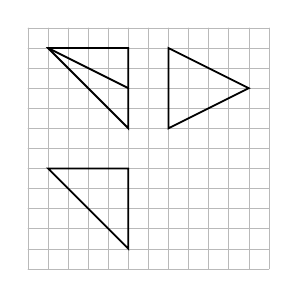
\begin{tikzpicture}[x=2.55mm,y=2.55mm,line cap=round]
  \draw[step=1,gray!55,line width=.18pt] (0,0) grid (12,12);
  % 左上投影：两条斜边从同一顶点出发。
  \draw[line width=.65pt] (1,11)--(5,11)--(5,7)--cycle;
  \draw[line width=.65pt] (1,11)--(5,9);
  % 右上投影：指向右侧的三角形投影。
  \draw[line width=.65pt] (7,11)--(11,9)--(7,7)--cycle;
  \draw[line width=.65pt] (7,11)--(7,7);
  % 左下投影：斜线三角形。
  \draw[line width=.65pt] (1,5)--(5,5)--(5,1)--cycle;
\end{tikzpicture}
\end{center}
\nopagebreak[4]
（A）$6\sqrt2$　　（B）$6$　　（C）$4\sqrt2$　　（D）$4$

\end{question}
\gkpart{二、填空题}

\begin{question}
\gkti{13}$(x-y)^8(x+y)^8$ 的展开式中 $x^2y^7$ 的系数为\gkblank{}。（用数字填写答案）

\end{question}
\begin{question}
\gkti{14}甲、乙、丙三位同学被问到是否去过 $A,B,C$ 三个城市时，甲说：我去过的城市比乙多，但没去过 $B$ 城市；乙说：我没去过 $C$ 城市；丙说：我们三人去过同一个城市。由此可判断乙去过的城市为\gkblank{}。

\end{question}
\begin{question}
\gkti{15}已知 $A,B,C$ 是圆 $O$ 上的三点，若 $\overrightarrow{AO}=\dfrac12(\overrightarrow{AB}+\overrightarrow{AC})$，则 $\overrightarrow{AB}$ 与 $\overrightarrow{AC}$ 的夹角为\gkblank{}。

\end{question}
\begin{question}
\gkti{16}已知 $a,b,c$ 分别为 $\triangle ABC$ 的三个内角 $A,B,C$ 的对边，$a=2$，且 $(2+b)(\sin A-\sin B)=(c-b)\sin C$，则 $\triangle ABC$ 面积的最大值为\gkblank{}。

\end{question}
\gkpart{三、解答题}

\begin{question}
\gkti{17}已知数列 $\{a_n\}$ 的前 $n$ 项和为 $S_n$，$a_1=1$，$a_n\ne0$，$a_na_{n+1}=\lambda S_n-1$，其中 $\lambda$ 为常数。

(1) 证明：$a_{n+2}-a_n=\lambda$；

(2) 是否存在 $\lambda$，使得 $\{a_n\}$ 为等差数列？并说明理由。

\par\medskip

*以下续自固定源 PDF 第 2 页（印刷页 900）。*

\Needspace{0.4\textheight}
\end{question}
\begin{question}
\gkti{18}从某企业生产的某种产品中抽取 $500$ 件，测量这些产品的一项质量指标值，由测量结果得如下频率分布直方图：
\nopagebreak[4]
\begin{center}% 2014 全国卷Ⅰ理科第 18 题：频率/组距直方图，保留断轴、虚线引导及七个空心柱。
\begin{tikzpicture}[font=\scriptsize,>=Stealth,line cap=round]
  \draw[->,line width=.45pt] (0,0)--(9.35,0) node[right] {质量指标值};
  \draw[->,line width=.45pt] (0,-.18)--(0,4.08) node[above left,align=center] {频率\\组距};
  \draw[line width=.4pt] (.13,.10)--(.21,-.10)--(.29,.10)--(.37,-.10)--(.45,.10);
  \node[below=2pt] at (0,0) {$0$};
  \foreach \x/\lab in {1/165,2/175,3/185,4/195,5/205,6/215,7/225,8/235} \node[below=2pt] at (\x,0) {\lab};
  % 数据高度按统一比例映射；横坐标每单位为一个组距 10。
  \draw (1,0) rectangle (2,.24); \draw (2,0) rectangle (3,1.08); \draw (3,0) rectangle (4,2.64);
  \draw (4,0) rectangle (5,3.96); \draw (5,0) rectangle (6,2.88); \draw (6,0) rectangle (7,.96); \draw (7,0) rectangle (8,.24);
  \foreach \y/\lab/\to in {.24/.002/8,.96/.008/7,1.08/.009/3,2.64/.022/4,2.88/.024/6,3.96/.033/5}
    {\draw[dashed,line width=.3pt] (0,\y)--(\to,\y); \node[left=2pt] at (0,\y) {\lab};}
\end{tikzpicture}
\end{center}
\nopagebreak[4]
(1) 求这 $500$ 件产品质量指标值的样本平均数 $\bar x$ 和样本方差 $s^2$（同一组数据用该区间的中点值作代表）；

(2) 由频率分布直方图可以认为，这种产品的质量指标值 $Z$ 服从正态分布 $N(\mu,\sigma^2)$，其中 $\mu$ 近似为样本平均数 $\bar x$，$\sigma^2$ 近似为样本方差 $s^2$。

① 利用该正态分布，求 $P(187.8<Z<212.2)$；

② 某用户从该企业购买了 $100$ 件这种产品，记 $X$ 表示这 $100$ 件产品中质量指标值位于区间 $(187.8,212.2)$ 的产品件数，利用①的结果，求 $EX$。

附：$\sqrt{150}\approx12.2$。若 $Z\sim N(\mu,\sigma^2)$，则 $P(\mu-\sigma<Z<\mu+\sigma)=0.6826$，$P(\mu-2\sigma<Z<\mu+2\sigma)=0.9544$。

\Needspace{0.4\textheight}
\end{question}
\begin{question}
\gkti{19}如图，三棱柱 $ABC-A_1B_1C_1$ 中，侧面 $BB_1C_1C$ 为菱形，$AB\perp B_1C$。
\nopagebreak[4]
\begin{center}% 2014 全国卷Ⅰ理科第 19 题：三棱柱；短虚线为经过隐藏顶点 C 的棱。
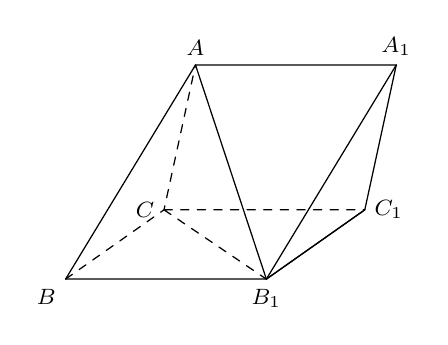
\begin{tikzpicture}[font=\footnotesize,line width=.45pt,line cap=round,line join=round]
  \coordinate (B) at (0,0); \coordinate (B1) at (2.55,0); \coordinate (C) at (1.25,.88); \coordinate (C1) at (3.80,.88);
  \coordinate (A) at (1.65,2.72); \coordinate (A1) at (4.20,2.72);
  \draw (B)--(A)--(A1)--(B1)--cycle; \draw (A1)--(C1)--(B1); \draw (A)--(B1); \draw (B1)--(C1);
  \draw[dashed] (B)--(C)--(A) (C)--(C1) (C)--(B1);
  \node[below left] at (B) {$B$}; \node[below] at (B1) {$B_1$}; \node[left] at (C) {$C$}; \node[right] at (C1) {$C_1$};
  \node[above] at (A) {$A$}; \node[above] at (A1) {$A_1$};
\end{tikzpicture}
\end{center}
\nopagebreak[4]
(1) 证明：$AC=AB_1$；

(2) 若 $AC\perp AB_1$，$\angle CBB_1=60^\circ$，$AB=BC$，求二面角 $A-A_1B_1-C_1$ 的余弦值。

\end{question}
\begin{question}
\gkti{20}已知点 $A(0,-2)$，椭圆 $E:\dfrac{x^2}{a^2}+\dfrac{y^2}{b^2}=1 (a>b>0)$ 的离心率为 $\dfrac{\sqrt3}{2}$，$F$ 是椭圆的右焦点，直线 $AF$ 的斜率为 $\dfrac{2\sqrt3}{3}$，$O$ 为坐标原点。

(1) 求 $E$ 的方程；

(2) 设过点 $A$ 的动直线 $l$ 与 $E$ 相交于 $P,Q$ 两点，当 $\triangle OPQ$ 的面积最大时，求 $l$ 的方程。

\end{question}
\begin{question}
\gkti{21}设函数 $f(x)=ae^x\ln x+\dfrac{be^{x-1}}x$，曲线 $y=f(x)$ 在点 $(1,f(1))$ 处的切线方程为 $y=e(x-1)+2$。

(1) 求 $a,b$；

(2) 证明：$f(x)>1$。

\Needspace{0.4\textheight}
\end{question}
\begin{question}
\gkti{22}如图，四边形 $ABCD$ 是 $\odot O$ 的内接四边形，$AB$ 的延长线与 $DC$ 的延长线交于点 $E$，且 $CB=CE$。
\nopagebreak[4]
\begin{center}% 2014 全国卷Ⅰ理科第 22 题：圆内接四边形、AB/DC 延长交点 E 与辅助线 MC。
\begin{tikzpicture}[font=\footnotesize,line width=.45pt,line cap=round,line join=round]
  % These coordinates satisfy the source relations to rounding precision:
  % A,B,C,D lie on the circle, D,C,E are collinear, CB=CE, and MB=MC.
  \coordinate (O) at (0,0); \coordinate (A) at (-1.920000,-1.440000); \coordinate (D) at (.287077,2.382769);
  \coordinate (M) at ($ (A)!0.5!(D) $); \coordinate (B) at (1.920000,-1.440000); \coordinate (C) at (2.207077,-.942769); \coordinate (E) at (2.494153,-1.440000);
  \draw (O) circle (2.4); \draw (A)--(D)--(C)--(B)--cycle; \draw (A)--(E); \draw (D)--(E); \draw (M)--(C);
  \fill (O) circle (1.15pt); \node[below left] at (A) {$A$}; \node[below] at (B) {$B$}; \node[right] at (C) {$C$};
  \node[above] at (D) {$D$}; \node[right] at (E) {$E$}; \node[left] at (M) {$M$}; \node[below left] at (O) {$O$};
\end{tikzpicture}
\end{center}
\nopagebreak[4]
(1) 证明：$\angle D=\angle E$；

(2) 设 $AD$ 不是 $\odot O$ 的直径，$AD$ 的中点为 $M$，且 $MB=MC$，证明：$\triangle ADE$ 为等边三角形。

\end{question}
\begin{question}
\gkti{23}已知曲线 $C:\dfrac{x^2}{4}+\dfrac{y^2}{9}=1$，直线 $l:\begin{cases}x=2+t,\\y=2-2t,\end{cases}$（$t$ 为参数）。

(1) 写出曲线 $C$ 的参数方程，直线 $l$ 的普通方程；

(2) 过曲线 $C$ 上任一点 $P$ 作与 $l$ 夹角为 $30^\circ$ 的直线，交 $l$ 于点 $A$，求 $|PA|$ 的最大值与最小值。

\end{question}
\begin{question}
\gkti{24}若 $a>0,b>0$，且 $\dfrac1a+\dfrac1b=\sqrt{ab}$。

(1) 求 $a^3+b^3$ 的最小值；

(2) 是否存在 $a,b$，使得 $2a+3b=6$？并说明理由。

\end{question}